\setcounter{chapter}{2}
\chapter{Methods}

\section{Models}\label{sec:models}

It is important to distinguish between the two model-types used in this thesis. This section intends to explain both the general idea behind the model-types, and the specifics pertaining to the chosen models.

\subsection{Numerical Weather Prediction - model}\label{sec:nwp}

A \acrfull{nwp}-model uses observational data as input to create an analysis for the current atmospheric state. This is done such that the model is run with the best estimate of the atmosphere . When the model then runs it advances in time, with a given timestep. This advance is done by solving the governing equations to calculate the next state of the atmosphere.This state is then recorded at fixed intervals (hourly for \acrshort{meps}) and this predicted/forecasted state is what constitutes a weather forecast. Operational \acrshort{nwp}-models are often updated when model upgrades are ready, so models for different time periods can be using different physics schemes. Modern \acrshort{nwp}-models also utilize perturbed ensemble-members. This is done by having a control run use the original observational data, and then making small (inside of the observational uncertainty range) changes or perturbations to the initial state. This could also include changes to the model itself (e.g. \cite{toth1993}). Each run is then a member in the whole ensemble, and the ensemble as a whole is meant to represent a range of possible outcomes from the observed starting state.

\subsubsection{MEPS}\label{sec:meps}

The operational \acrfull{meps}\footnote{Note that in February 2020, both the format and frequency of model runs for \acrfull{meps} was changed considerably, operational here refers to the model-runs from 2016-2019} model uses a timestep of $75s$, a horizontal grid with a $2.5x2.5$km  resolution, with $65$-vertical model levels in the HARMONE-AROME system (\cite{bengtsson2017}). Archived data for this model-setup is available for the period 2016 to 2019 at thredds.met.no.

\subsection{Reanalysis - model}\label{sec:ra}

A reanalysis differs from an operational \acrshort{nwp}-model in that it uses a fixed version of an \acrshort{nwp}-model on historical weather observations. This is done to create the best possible historical weather data, by turning point and field observations into a complete gridded archive of historical weather. Reanalysis models may also be run with pertubated ensembles, to capture variation between the times when observational data is considered.

\subsubsection{ERA5}\label{sec:era5}
The \acrfull{era5} dataset is created by the \acrfull{ecmwf} and provides hourly data, in $31x31$km grids, with $137$ vertical model-levels. The data ranges from $1979$ to and including $2019$ (It is continually updated as I write this, so it is probably updated beyond 2019). The observational data is assimilated in 12-hour windows (\cite{hersbach2018}).
This thesis utilizes the \acrshort{era5} dataset to create a set of climatologies and case-based atmospheric conditions, using the data reported on pressure levels.

\section{Data}\label{sec:data}

\subsection{Incidents from Avinor}\label{sec:avinordata}
For the purpose of this thesis have received a dataset from Avinor. This data included all reports on helicopter and plane incidents reported to Avinor pertaining to lightning. have filtered out cases where there was observed lightning in the area and not striking the aircraft, to prevent identifying "normal" lightning.

\begin{table}
    \begin{tabular}{ l|c|c|c|c|c} 
    		&Total cases & Height info & Position & Reported temp. (\acrshort{oat}) & After November 2016\\
     		\hline
     		Helicopters &$40$ & $37$ & $24$ & $12$&$19$\\
     		Fixed-wing &$256$ & $217$ & $256$ & $1$&$58$\\ 
     		\hline
     		Total &$296$ &$254$ & $280$ & $13$&$77$\\ 
     		\hline
    \end{tabular}
    \caption{Data available for each case in the Avinor-dataset. Note that there is one helicopter case where height is not known, but position is. }
    \label{tab:avinor}
\end{table}

\subsection{Meteorological aerodrome report}\label{sec:metar}
\acrlong{metar} is a report given every half hour at airports throughout the world, to ensure that the weather allows flying. This is a subjective report by trained personnel of the current weather. 

\begin{table}
    \centering
    \begin{tabular}{r|l}
        METAR-code & Description \\
        \hline
        CB & Cumulonimbus cloud \\
        TCU & Towering Cumulus cloud\\
        RA & Rain \\
        SN & Snow  \\
        GS & Hail \\
        GR & Graupel \\
        SH & Showers    \\
        VCSH & Showers in vicinity \\
        FEW & Few clouds (1-2/8)\\
        SCT & Scattered clouds (3-4/8)\\
        BKN & Broken clouds (5-7/8)\\
        OVC & Overcast (8/8)\\
    \end{tabular}
    \caption{METAR-codes for reporting weather phenomena. The last four categories includes a numerical value for how much of the cloud is covered by clouds, OVC refers to total cloud cover, FEW refers to one to two eights of sky is cloud }
    \label{tab:METAR-table}
\end{table}

\section{Statistics}\label{sec:statistics}

\subsection{Nearest neighbour maxima/minima}\label{sec:nearestneigh}

\subsection{Data average - Mean}\label{sec:mean}
Climatologies.

\subsection{Data variation - Standard deviation}\label{sec:std}

\subsection{Difference in data - Mean Absolute Difference}\label{sec:mad}

\section{Post - processing}\label{sec:pp}
This thesis does not perform any model-runs but instead focus on already produced model-products. This after the fact processing of data is referred to as post-processing. The \acrshort{hti} is a post-processing product, it does not result from a subroutine run during the model-operation. Instead it is made by assessing the output from the model. This section describe the how this is done operationally, and eventual problems with this philosophy.

\subsection{Interpolation}\label{sec:interpolation}

\begin{figure}
    \centering
    \begin{subfigure}[h]{0.45\textwidth}
    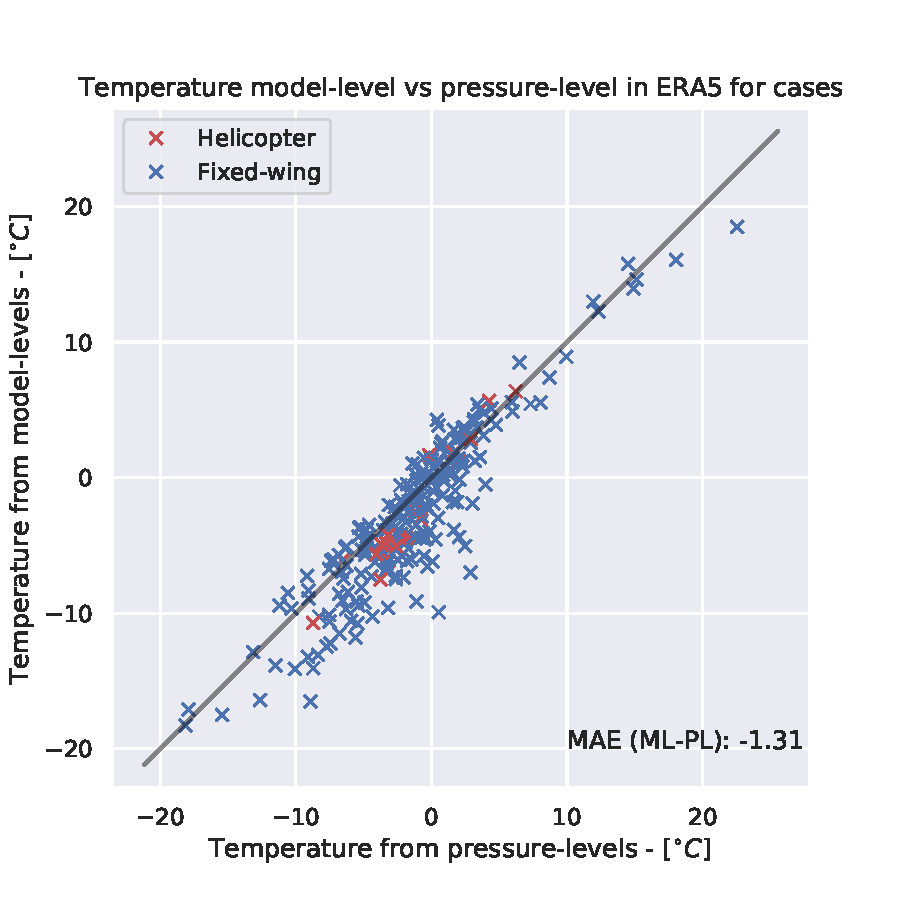
\includegraphics[width=\textwidth]{Figures/mlvspl.pdf}
    \caption{Scatter plot between model-level and pressure-level interpolation of temperature from ERA5, also printed on the figure: Mean Absolute Difference (MAD), showing model-level interpolation averagely colder than Pressure Level with $1.31^{\circ}$ Celsius.}
    \label{fig:mlvspltemp}
    \end{subfigure}
    \hfill
    \begin{subfigure}[h]{0.45\textwidth}
    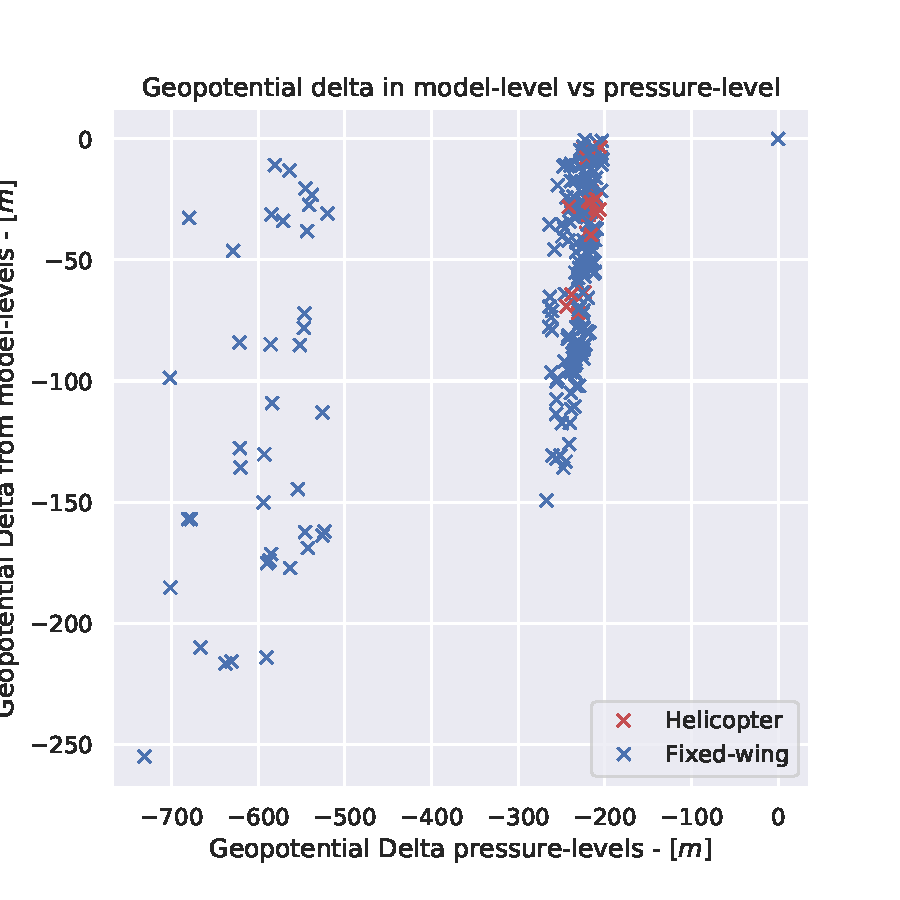
\includegraphics[width=\textwidth]{Figures/geopot.pdf}
    \caption{Scatter plot between model-level and pressure-level interpolation of geopotential height from ERA5.}
    \label{fig:mlvsplgeopot}
    \end{subfigure}
\end{figure}

% \begin{figure}
%     \centering
%     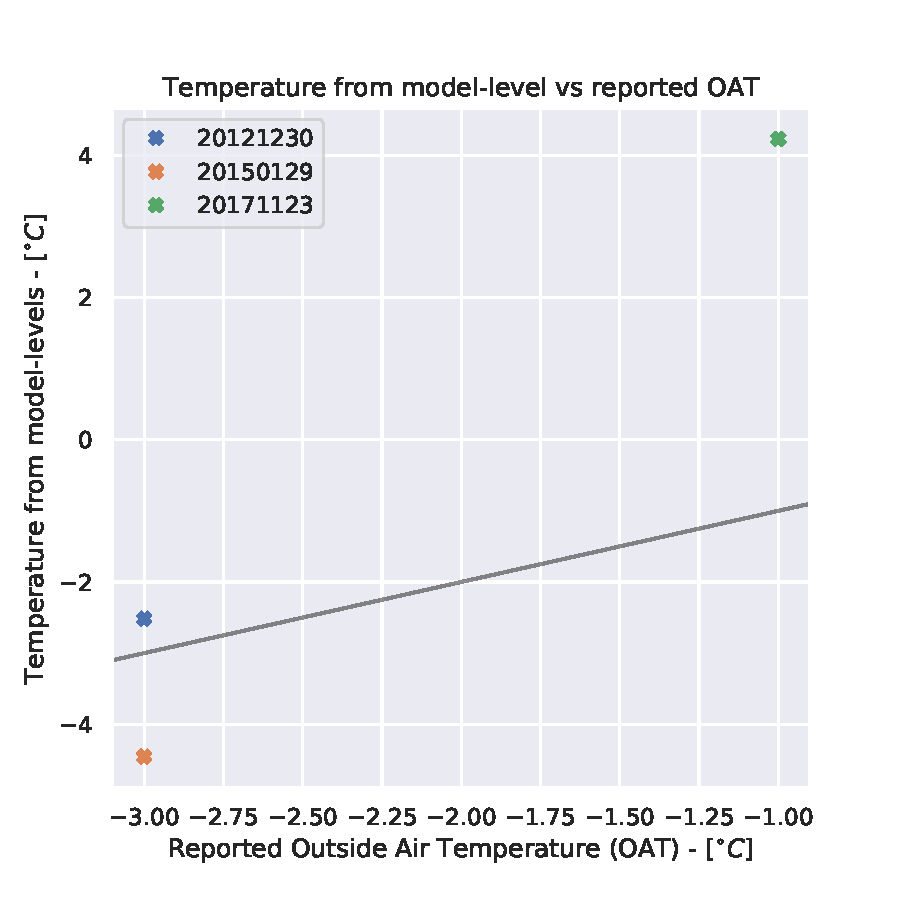
\includegraphics[height=0.4\textheight]{Figures/mlvsoat.pdf}
%     \caption{Scatterplot of between model-level interpolation for temperature from ERA5 against observed Outside Air Temperature}
%     \label{fig:mlvsoat}
% \end{figure}

% \begin{figure}
%     \centering
%     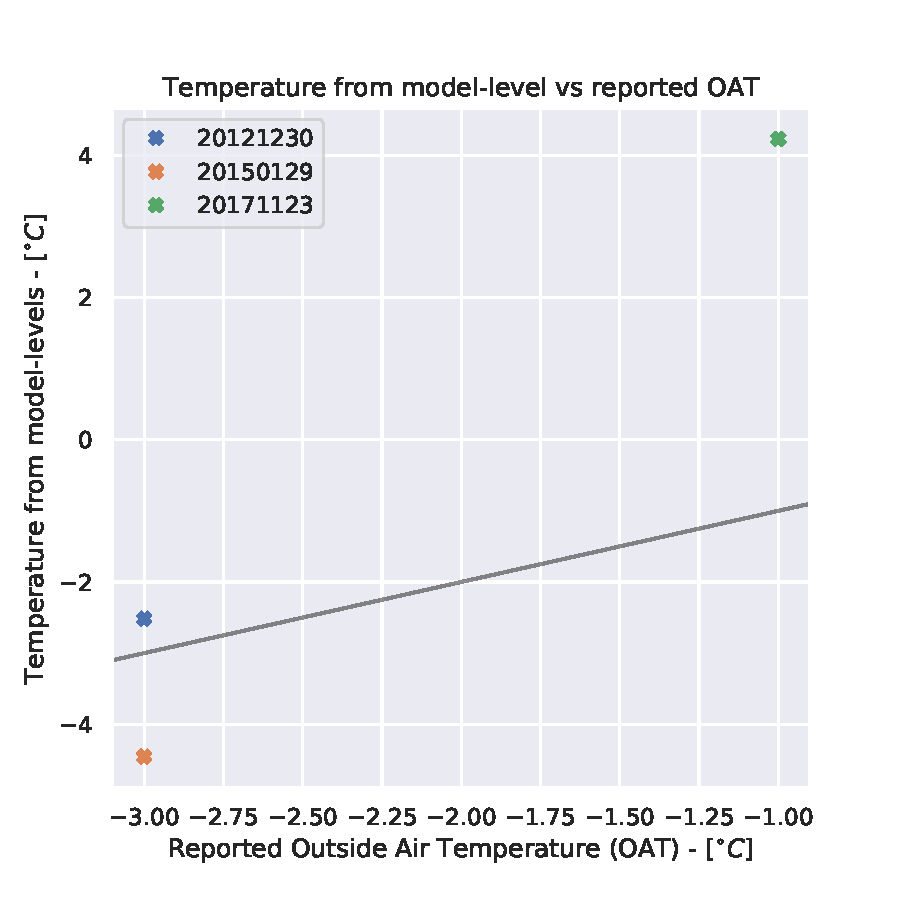
\includegraphics[height=0.4\textheight]{Figures/mlvsoat.pdf}
%     \caption{Scatterplot of pressure-level interpolation for temperature from ERA5 against observed Outside Air Temperature}
%     \label{fig:plvsoat}
% \end{figure}

\subsection{Helicopter Trigger Index }\label{sec:hti}

(\cite{lande1999}) looked at the common atmospheric conditions present for a \acrshort{htl}:
\begin{itemize}
 \item \acrfull{oat} at flight level near freezing point 
 \item frozen precipitation, as snow, ice and graupel.
 \item inside of or directly below clouds.
 \item within 5 nautical miles of a Cumulonimbus cloud.
\end{itemize}

The operational forecast as of today is based on findings by \cite{hardwick1999} and \cite{wilkinson2013}. It assigns a risk or \acrfull{hti} in percentage based on four meteorological factors:
\begin{itemize}
    \item Vertical wind speed in the altitude that helicopters generally fly in.
    \begin{itemize}
        \item Positive (Upward) vertical wind gives a non-zero value.
        \item Negative (downward) vertical wind gives 0 value.
    \end{itemize}
    \item Temperature at the altitude that helicopters generally fly in.
    \begin{itemize}
        \item Temperatures in the $[0,-6] ^{\circ}C$ range gives non-zero value. 
        \item 0 for temperatures outside this range
    \end{itemize}
    \item Total precipitation during the last hour.
    \begin{itemize}
        \item Linear from $0\frac{mm}{hr}$ with 0 value to full value at $0.75\frac{mm}{hr}$ precipitation intensity.
    \end{itemize}
    \item Amount of low clouds in the surrounding area.
    \begin{itemize}
        \item Value is calculated by the difference in neighbourhood maximum cloud cover and neighbourhood minimum cloud cover. Full cloud cover gives 0 value, no clouds gives 0 value.
    \end{itemize} 

\end{itemize}
The \acrshort{hti} is the sum of these four subrisks, \[\text{HTI} = \frac{\text{Vertical Wind}}{4} + \frac{\text{Temperature}}{4} + \frac{\text{Precipitation}}{4} +\frac{\text{Cloud}}{4}\] equally weighted, such that \acrshort{hti} is valued in the range $[0,100]\%$. The index is categorized in four different classes of severity, from no danger (White) to very high risk (Red). (See figure \ref{fig:hti}).
\begin{itemize}
    \item White: $HTI < 0.73$
    \item Yellow: $0.73 \leq HTI < 0.90 $
    \item Orange: $0.90 \leq HTI < 0.99 $
    \item Red: $0.99 \leq HTI $
\end{itemize}
The severity-categories are based on discussion with the helicopter operators in Norway (Bristow and CHC), and are changed if deemed necessary after the yearly evaluation of the season. \acrshort{hti} is not based on a regression analysis, but rather a subjective review of the earlier cases of incidents.
\begin{figure}
    \centering
    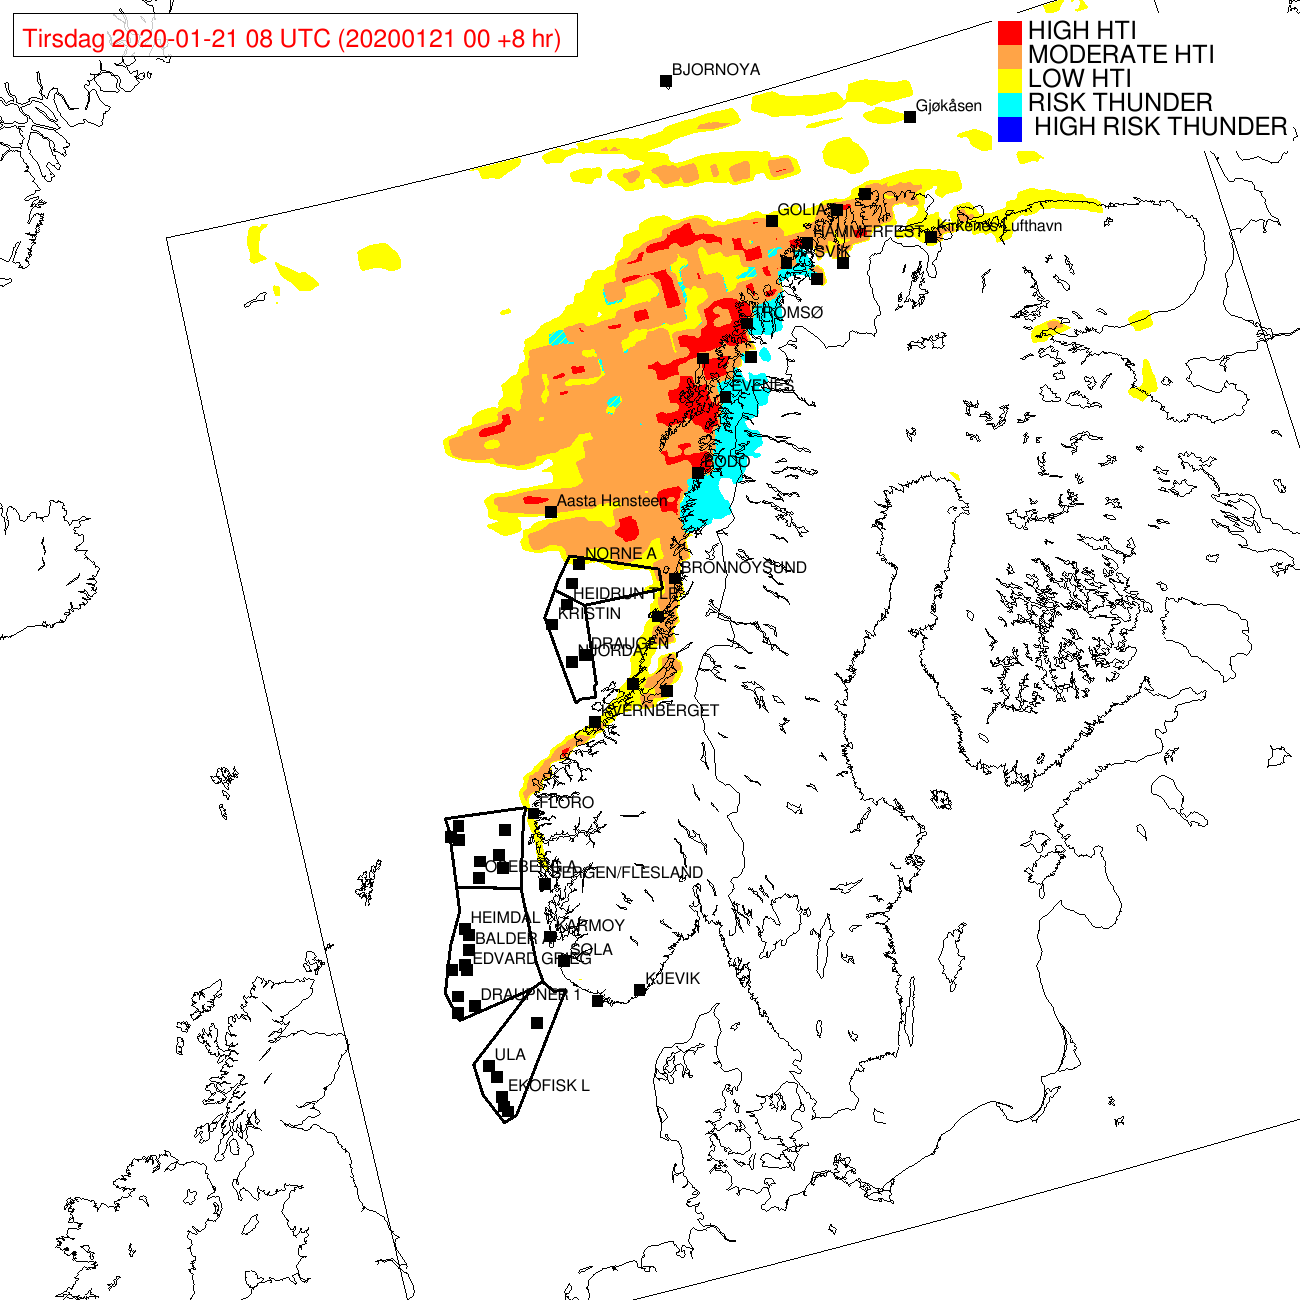
\includegraphics[width=\textwidth]{Figures/hti.png}
    \caption{Screenshot from https://www.ippc.no for 21. of January 2020, showing the HTI-forecast with 8 hour lead-time after midnight. The blue thunder-cells show another forecast-product from MET, forecasting risk for natural lightning. A plane was hit by lightning, and was therefore diverted from flying into Bodø during this forecasts valid time. }
    \label{fig:hti}
\end{figure}

\subsubsection{Decomposition of HTI}\label{decomposition}

To further investigate the effect of each parameter, the \acrshort{hti} is decomposed into subindices, one for each parameter. This allows 